%\beginsupplement

\renewcommand{\thefigure}{A\arabic{figure}}
\setcounter{figure}{0}
\renewcommand{\thetable}{A\arabic{table}}
\setcounter{table}{0}

\section{Supplementary Data}
\label{supplinfo}


\subsection{Intermolecular potentials}
\label{sec:SIpotentials}

The isoPAHAP and curPAHIP potentials take the following form, 
%
\begin{equation}
\label{eqn:isoPAHAP}
U_{ab} = K \exp \left[ - \alpha_{ab} \left( R_{ab} - \rho_{ab} \right) \right] - \left[ 1 - \exp \left( - \beta R_{ab} \right) \sum_{k=0}^{6} \frac{ \left( \beta R_{ab} \right) ^{k}}{k!} \right] \frac{C_{6,ab}}{R_{ab}^{6}} + \frac{q_{a} q_{b}}{R_{ab}},
\end{equation}
%
where the first term is the short-range term in the Born--Mayer form, the second term is the dispersion term damped by the Tang-Toennies damping function \citep{Tang1984}, and the third is the point charge electrostatic term. $U$ denotes the interaction energy, $K$ sets the energy unit of this term and will be taken to be $0.001$ hartree in this work, $\alpha$ is the hardness parameter in the Born--Mayer term, $R_{ab}$ is the atom-atom separation where $a$ and $b$ denote atomic sites within a molecule, $\rho_{ab}$ is a shape parameter, $\beta$ is the damping coefficient, $C_{6,ab}$ is a dispersion coefficient, and $q$ is the atomic point charge. Further details about the parametrisation and form of the isoPAHAP potential can be found in \citet{totton2010first}.

Table~\ref{table:curPAHAPparams} provides the parameters of the curPAHIP intermolecular potential. 
%
\begin{table}[h!tb]
\centering
\caption{Parameters of curPAHIP in a.u.}
\label{table:curPAHAPparams}
\begin{tabular}{cccc}
\hline
Atom pair & $\rho $   & $\alpha$ 	&	$C_{6}$  \\ \hline
C C       & 5.6563 & 1.8783 & 30.282  \\
C H       & 4.9320 & 1.7560 & 12.604  \\
H H       & 4.1187 & 1.4043 & 5.2179  \\ \hline
$\beta = 1.50$ a.u.
\end{tabular}
\end{table}

The following interaction parameters are used to describe systems containing \ce{K+}: $\sigma = 9.64$ and $\epsilon = 3.43\times10^{-8}$ a.u. Further information on the development and parameters of the curPAHIP potential can be found in \citet{bowal2019ion}.


\subsection{Molecule descriptions}
\label{sec:SImoleculedesc}
Corannulene (A) geometry (x, y, z in nm) and charges, taken from \citet{bowal2019ion}, are provided below.
%
\begin{verbatim}
35 
CORANNULENE with curPAHIP charges
C     0.103   0.064   0.085    0.020  
C     0.093  -0.078   0.085    0.020  
C    -0.045  -0.112   0.085    0.020  
C    -0.121   0.008   0.085    0.020  
C    -0.030   0.117   0.085    0.020  
C     0.205   0.129   0.022    0.177  
C     0.310   0.049  -0.032   -0.201 
C     0.300  -0.090  -0.032   -0.201 
C     0.187  -0.156   0.022    0.177  
C     0.143  -0.279  -0.032   -0.201 
C     0.007  -0.313  -0.033   -0.201 
C    -0.090  -0.225   0.022    0.177  
C    -0.242   0.016   0.022    0.177  
C    -0.296  -0.103  -0.032   -0.201 
C    -0.222  -0.222  -0.032   -0.201 
C    -0.280   0.142  -0.031   -0.201 
C    -0.190   0.250  -0.031   -0.201 
C    -0.059   0.235   0.023    0.177  
C     0.049   0.310  -0.032   -0.201 
C     0.178   0.258  -0.032   -0.201 
H    -0.221   0.345  -0.072    0.133  
H     0.031   0.408  -0.072    0.133  
H     0.259   0.317  -0.073    0.133  
H     0.398   0.097  -0.072    0.133  
H     0.380  -0.149  -0.075    0.133  
H     0.215  -0.348  -0.073    0.133  
H    -0.024  -0.408  -0.074    0.133  
H    -0.265  -0.312  -0.073    0.133  
H    -0.396  -0.103  -0.074    0.133  
H    -0.378   0.155  -0.073    0.133  
X     0.103   0.064   0.132   -0.063 
X     0.093  -0.078   0.132   -0.063 
X    -0.045  -0.113   0.132   -0.063 
X    -0.121   0.008   0.133   -0.063 
X    -0.030   0.117   0.133   -0.063
\end{verbatim}

The following atomic coordinates (in nm) and charges are used in this work for the \ce{C42H14} molecule (B).
%
\begin{verbatim}
66
2PENT15RING MOLECULE with curPAHIP charges
C    -0.200   0.000   0.135   -0.309
C    -0.317   0.000   0.043    0.425
C    -0.365  -0.132  -0.016   -0.126
C    -0.126  -0.124   0.159    0.041
C    -0.126   0.124   0.158    0.041
C     0.014   0.124   0.176    0.070
C     0.093   0.000   0.174   -0.190
C     0.014  -0.125   0.177    0.070
C     0.065  -0.244   0.122   -0.117
C    -0.486  -0.127  -0.098   -0.225
C    -0.543   0.000  -0.139    0.010
C    -0.486   0.127  -0.096   -0.225
C    -0.365   0.131  -0.016   -0.126
C    -0.277   0.252  -0.001    0.253
C    -0.162   0.242   0.091   -0.109
C    -0.044   0.318   0.073    0.039
C     0.065   0.244   0.122   -0.117
C     0.197   0.251   0.059    0.008
C     0.282   0.128   0.056    0.150
C     0.229   0.000   0.111    0.038
C    -0.029   0.421  -0.031    0.157
C     0.110   0.463  -0.060   -0.365
C     0.219   0.365  -0.036    0.346
C    -0.154   0.458  -0.100   -0.163
C    -0.275   0.373  -0.088   -0.210
C     0.284  -0.130   0.058    0.150
C     0.198  -0.252   0.060    0.008
C     0.401   0.126  -0.034   -0.116
C     0.347   0.366  -0.109   -0.392
C     0.435   0.249  -0.107   -0.017
C     0.220  -0.365  -0.036    0.346
H    -0.526   0.219  -0.137    0.128
H    -0.629   0.001  -0.205    0.090
H     0.369   0.449  -0.175    0.162
H     0.127   0.540  -0.134    0.161
H    -0.153   0.535  -0.176    0.116
H    -0.356   0.391  -0.157    0.133
C     0.402  -0.128  -0.032   -0.116
C     0.473   0.000  -0.054   -0.115
C     0.352  -0.369  -0.100   -0.392
C     0.437  -0.250  -0.105   -0.017
C    -0.278  -0.253   0.001    0.253
C    -0.162  -0.243   0.092   -0.109
C    -0.044  -0.318   0.072    0.039
C    -0.030  -0.418  -0.035    0.157
C     0.109  -0.458  -0.067   -0.365
C    -0.280  -0.378  -0.079   -0.210
C    -0.156  -0.455  -0.103   -0.163
H    -0.363  -0.398  -0.146    0.133
H    -0.153  -0.525  -0.186    0.116
H    -0.527  -0.218  -0.140    0.128
H     0.126  -0.534  -0.142    0.161
H     0.376  -0.453  -0.165    0.162
H     0.520  -0.246  -0.173    0.104
H     0.558  -0.001  -0.121    0.129
H     0.523   0.248  -0.171    0.104
X    -0.132   0.148   0.204    0.044
X    -0.170   0.266   0.137   -0.107
X    -0.051   0.340   0.119    0.041
X     0.060   0.267   0.169   -0.115
X     0.008   0.148   0.223    0.072
X    -0.050  -0.341   0.118    0.041
X    -0.169  -0.267   0.138   -0.107
X    -0.132  -0.148   0.205    0.044
X     0.060  -0.267   0.168   -0.115
X     0.009  -0.148   0.223    0.072

\end{verbatim}

In both molecules, the element X represents the virtual mass-less atoms used to describe the flexoelectric effect, which are held above and parallel to the pentagon ring using intramolecular forces.

\subsection{Replica Exchange Molecular Dynamics simulation parameters}
\label{secSI:REMDtemps}
%
Replica temperatures for REMD simulations were selected using an exponential temperature distribution
\begin{equation}
\label{eqn:replica_temp_dist}
T_{w} = T_{0}\exp(qw)
\end{equation}
where $T_w$ refers to the temperature (in K) at replica $w$, $T_0$ is the temperature (K) at replica $0$, and $q$ is a parameter which achieves the desired temperature range. 

The temperature ranges are selected to encompass both solid- and liquid-like configurations. These temperature ranges differ with the molecular composition of the cluster, since constituent molecule sizes determine the temperature at which a cluster is liquid- or solid-like. The smallest molecule present determines the lower temperature bound, with A or C molecules at 200 K and B molecules at 400 K. Similarly the largest molecule present determines the upper temperature bound, with A or C molecules at $\ge 800$ K and B molecules at $\ge 1600$ K. 

The $w$ and $q$ parameters, shown in Table~\ref{tableSI:REMDparams}, are selected for each cluster system to allow satisfactory exchange between replicas (discussed further below) using these temperature ranges.
%
\begin{table}[ht]
\centering
\caption{Replica temperature selection parameters %and resulting average exchange acceptance values 
for cPAH clusters considered in this work.}
\label{tableSI:REMDparams}
\begin{tabular}{lcc}%c}
\hline
Cluster & $q$ & $w$ \\ \hline %& Acceptance 
$\text{A}_{\text{25}}$ & 0.054 & 0-26 \\ %& 0.28-0.30
$\text{A}_{\text{40}}$ & 0.050 & 0-29 \\ % & 0.19-0.24 
$\text{A}_{\text{50}}$ & 0.040 & 0-35 \\ % & 0.24-0.28 
$\text{A}_{\text{100}}$ & 0.025 & 0-59 \\ % & 0.28-0.35 
$\text{A}_{\text{200}}$ & 0.017 & 0-86 \\ \hline % & 0.30-0.37
$\text{B}_{\text{25}}$ & 0.045 & 0-32 \\ % & 0.20-0.26 
$\text{B}_{\text{40}}$ & 0.032 & 0-44 \\ % & 0.13-0.41 
$\text{B}_{\text{50}}$ & 0.030 & 0-47 \\ % & 0.22-0.28 
$\text{B}_{\text{100}}$ & 0.024 & 0-59 \\ \hline % & 0.10-0.25 
$\text{A}_{\text{20}}\text{B}_{\text{20}}$ & 0.030 & 0-71 \\ % & 0.35-0.42 
$\text{A}_{\text{50}}\text{B}_{\text{50}}$ & 0.025 & 0-83 \\ % & 0.20-0.30 
$\text{A}_{\text{30}}\text{B}_{\text{10}}$ & 0.036 & 0-59 \\ % & 0.30-0.38 
$\text{A}_{\text{10}}\text{B}_{\text{30}}$ & 0.028 & 0-74 \\ \hline % & 0.33-0.41 
$\text{B}_{\text{40}}\text{K}_{\text{1}}$ & 0.030 & 0-47 \\ % & 0.32-0.40 
$\text{A}_{\text{40}}\text{K}_{\text{1}}$ & 0.050 & 0-29 \\ % & 0.21-0.23 
$\text{A}_{\text{40}}\text{K}_{\text{2}}$ & 0.050 & 0-29 \\ \hline % & 0.21-0.23 
\end{tabular}
\end{table}
%

The effectiveness of an REMD simulation relies on the proper exchange of states between replicas so that the low temperature states are able to sample the high temperature configurations and vice versa. Replica exchange acceptance is a good indication of the movement between replicas and is a common indicator of simulation performance. Consistent acceptance values across indicate a good temperature selection for the system studied and an exchange acceptance of approximately $0.2$ is found empirically and theoretically to provide the best accuracy for a given computational time \cite{Rathore2005,Kone}. Exchange acceptances for simulations conducted in this work have an average between $0.20$ and $0.35$ with small system ranges, which indicates robust replica exchange with a good balance between equilibration within replicas and exchange between replicas. Replica exchange attempts are made every 100 fs, since frequent exchanges are shown to increase efficiency without affecting the ensemble being sampled \cite{sindhikara2008exchange,sindhikara2010exchange}.

\subsection{Calculation of radial distances and coordination numbers}
\label{secSI:raddist_CN_eqns}
%
Average radial distances and coordination numbers are calculated to provide insight into molecular arrangements and cluster structure. The average radial distance of molecule type $k$, $r_{k}$, is calculated using the following equation:
\begin{equation}
    r_{k} = \frac{1}{N_{k}}\sum_{m \in I_{k}}R_{m}
\end{equation}
where $N_{k}$ is the number of molecules within $k \in \{\text{A},\text{B}\}$, referring to the corannulene and \ce{C42H14} molecule types, $I_{k}$ is the set of molecule indices within $k$, and $R_{m}$ is the radial distance between the cluster geometric centre and the geometric centre of molecule $m$. In this work, radial distances are calculated considering all atoms in the system.

The coordination number of molecule type $k$, $CN_{k},$ provides the average number of molecules within a distance $R^{(\text{cutoff})}$. This is calculated as the average of the cumulative radial distribution function integrated over the centre of the cluster (set as the origin at 0) to a maximum cut-off radial distance, $R^{(\text{cutoff})}$:
\begin{equation}
    CN_{k}(R^{(\text{cut-off})}) = \frac{1}{N_{k}} \sum_{m \in I_{k}} \int\limits_{0}^{R^{(\text{cut-off})}}  \sum_{j=1}^{N_{\text{total}}} \delta(D_{mj} - R) dR
\end{equation}
$k \in \{\text{A}, \text{B}, \text{total}\}$ refers to the A molecules, B molecules, and all curved molecules within the cluster, respectively. $D_{mj}$ is the distance between the geometric centres of molecules $m$ and $j$. 
This provides $CN$ values from zero to two, corresponding to an isolated molecule and a molecule sandwiched between two others, respectively.

%\subsection{Position restraint negligibility at low temperature}

%\subsection{Simulation length equilibration check}
%Energies and radial distances don't change significantly when comparing eqm result from 3ns simulation (final 1ns) or 1ns simulation (final 500ps)
%Percent error of intermolecular energies are less than 0.2\%
%Percent error of radial distances are less than 3.5\%

\subsection{Corannulene crystal structure}
\label{secSI:corannulenecrystal}
Several of the structural metrics used in this paper were applied to the known crystal structure of corannulene in order to provide a benchmark. 
%Further comparison is made with a 2pent15ring system and published large cPAH systems - Actually this should be included in the discussion sections of the paper I think.
As early as 1975, it was shown through X-ray analysis that corannulene crystallises in a close-packed structure mostly stabilised through CH-$pi$ interactions, in space group \textit{P}$2_{1}/c$ \cite{hanson1976crystal}.

A crystal structure containing 18 molecules, taken from The Cambridge Crystallographic Data Centre \cite{CORANN11unitcell}, provides an independent verification of the analyses used in this work as well as a known experimental structure useful for comparison. The average intermolecular spacing values are 0.57 nm, 0.72 nm, and 0.76 nm consider 1, 2, and 3 neighbouring molecules, respectively. The individual distances between corannulene monomers within the crystal structure calculated in this analysis are in excellent agreement with those reported in \citet{sanyal2014functional}. Figure~XX shows the crystal structure and alignment angles examined in this work.

%(using cut-off value of $R = 0.7$ nm)
%Intermolecular distances: 0.55 nm x 10, 0.61 nm x 6 (for first molecule); 0.61 x 2, 0.72 x 10, 0.73 x 2, 0.76 x 2, 0.78 x 2 (for second molecule), 0.72 x 2, 0.73 x 4, 0.76 x 8, 0.78 x 2, 0.82 x 2 (third molecule)... NOT SURE HOW TO SHOW THESE -> FOLLOW SAME PATTERN USED IN HOW I DISCUSS THIS IN THE PAPER (AVERAGE INTERMOLECULAR DISTS? - WOULD BE 0.57 NM FOR FIRST MOLECULE, ETC)
%
\begin{figure}[!tbh]
\centering
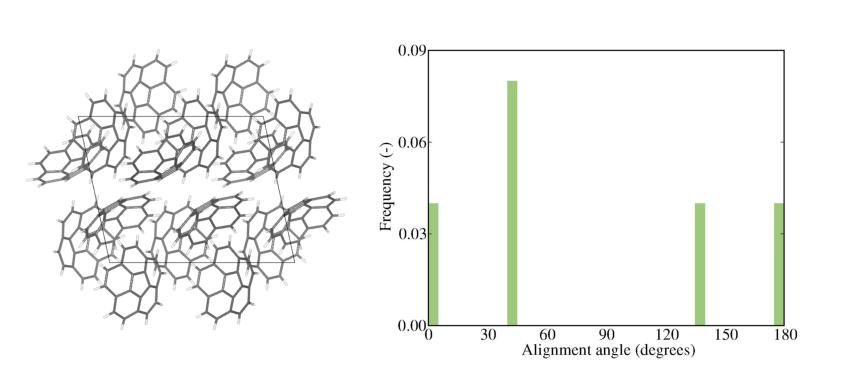
\includegraphics[width=0.65\linewidth]{Figures/corannulene_crystal.eps}
\caption{Snapshot of corannulene crystal structure (left) with alignment angle distribution (right).}
\label{figSI:corannulene_crystal}
\end{figure}
%

% add calculation of corannulene crystal structure CNs?

\subsection{Cut-off distance sensitivities}
\label{secSI:cutoffs}
The selection of the cut-off distance, $R$, influences the calculated average intermolecular distances, coordination numbers, and alignment angles.

Due to the molecular arrangements of the homogeneous A clusters (that is, sandwich-type stacking is not present), these results are the most sensitive to the selection of $R$.


Figure~\ref{figSI:alignmentangles_cutoffs} shows the alignment angle distributions for all homogeneous clusters using four different cut-off distances.  The influence of the cut-off distance is minimal in the B clusters, which show a very high proportion of molecules with at least one near neighbour at all cut-off distances.  At the higher cut-off distances, a second peak corresponding to further molecule layers (ie not the nearest neighbours alone) appears.  The A clusters show relatively similar angle distributions across the cut-off distances, although the percent of molecules with a near neighbour increases dramatically between $R=0.5$ nm and $R=0.6$ nm.  
%
\begin{figure}[!tbh]
\centering
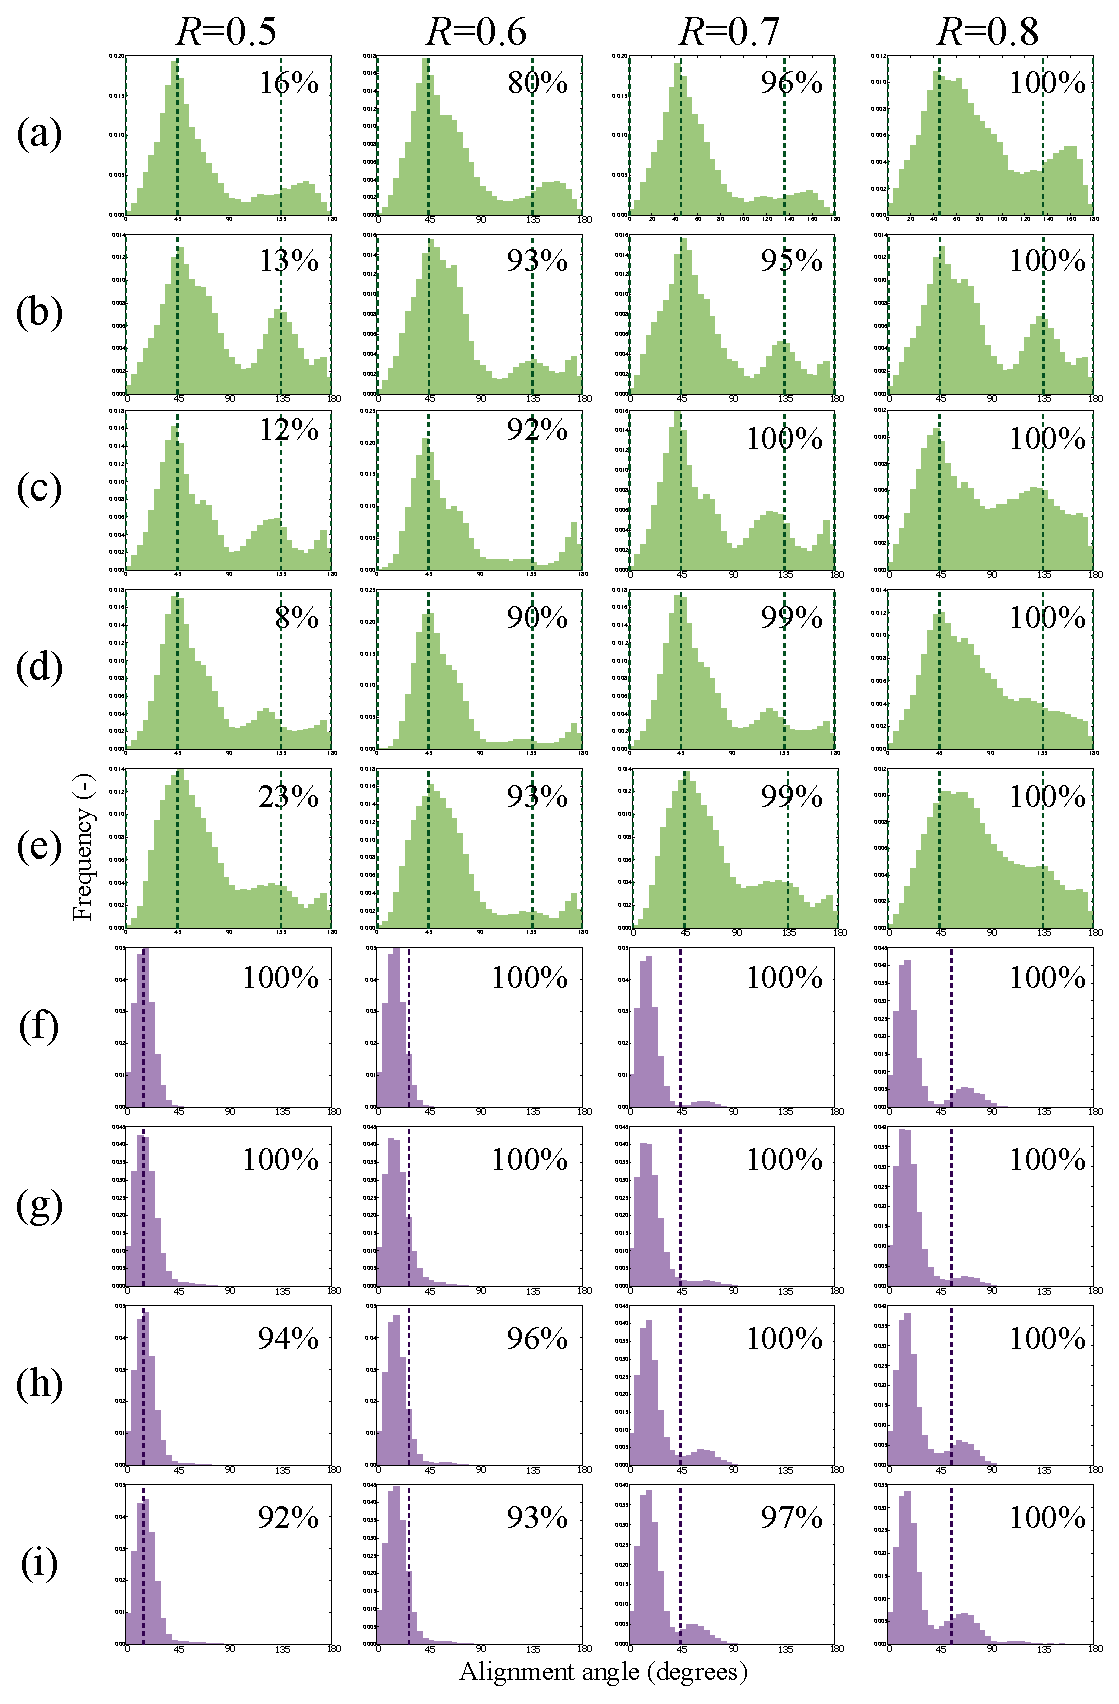
\includegraphics[width=0.85\linewidth]{Figures/AlignmentAnglesCutoffAssessment_SI.eps}
\caption{Alignment angle distributions at different cut-off distances, $R$, in nm for the following clusters: (a) ann\_25, (b) ann\_40, (c) ann\_50, (d) ann\_100, (e) ann\_200, (f) two\_25, (g) two\_40, (h) two\_50, (i) two\_100. Dashed lines correspond to the A crystal structure (for (a)-(e)) and the minimised B dimer (for (f)-(i)). Percent values in the upper right hand corners of each angle distribution refer to the percent of molecules within the cluster that have at least one near neighbour.}
\label{figSI:alignmentangles_cutoffs}
\end{figure}
%

- Include figure of CN histograms with r=0.5 for A and B

Note that for all systems, no neighbouring molecules are found using a cut-off distance of 0.4 nm or smaller.


Table~\ref{tableSI:intermolecdistscutoff} presents the average intermolecular distances of homogeneous clusters as a function of the cut-off distance used in analysis. For the corranulene molecule clusters, the cut-off distance selected influences the average intermolecular distance calculated.  Intuitively, an increase in the cut-off distance produces an increase in the average intermolecular distance, since the cut-off distance simply increases the range between 'neighbouring' molecules. At low cut-off values ($r = 0.5$ nm and $r = 0.6$ nm) very few molecule pairs exist and so these averages are not a clear picture of the true average intermolecular spacing throughout the cluster.  At $r = 0.7$ nm, the majority of molecules ($\ge 95$\%) have at least one near neighbour and therefore this provides the best indication of the cluster average.
% perhaps include the % of molecules that have a neighbour in each case?

In contrast, the cut-off distance does not have a large impact on the average intermolecular spacing of homogeneous B molecules. This highlights the highly stacked configuration of these molecules.




% 
\begin{table}[]
\centering
\caption{Average molecular intermolecular distance, in nm, for homogeneous clusters with varying cut-off values, $r$ in nm, used.}
\label{tableSI:intermolecdistscutoff}
\begin{tabular}{lcccc}
\hline
\multicolumn{1}{l}{\multirow{2}{*}{Cluster}} & \multicolumn{4}{c}{\multirow{1}{*}{Intermolecular distance}} \\
 & $r = 0.5$ & $r = 0.6$ & $r = 0.7$ & $r = 0.8$ \\ \hline
ann\_25 & 0.45 & 0.55 & 0.59 & 0.68 \\
ann\_40 & 0.45 & 0.55 & 0.59 & 0.67 \\
ann\_50 & 0.47 & 0.55 & 0.60 & 0.67 \\
ann\_100 & 0.48 & 0.55 & 0.59 & 0.68 \\
ann\_200 & 0.47 & 0.55 & 0.60 & 0.68 \\ \hline
two\_25 & 0.44 & 0.44 & 0.45 & 0.49 \\
two\_40 & 0.45 & 0.45 & 0.46 & 0.47 \\
two\_50 & 0.45 & 0.45 & 0.48 & 0.50 \\ 
two\_100 & 0.45 & 0.45 & 0.48 & 0.52 \\ \hline
%ann\_40\_Kion\_1 & 0.44 & 0.56 & 0.61 & 0.67 \\
%ann\_40\_Kion\_2 & 0.45 & 0.55 & 0.58 & 0.66 \\
%two\_40\_Kion\_1 & 0.46 & 0.46 & 0.48 & 0.53 \\ \hline
\end{tabular}
\end{table}
%





\subsection{Alignment angles - 100 molecule systems}
%
\begin{figure}[!tbh]
\centering
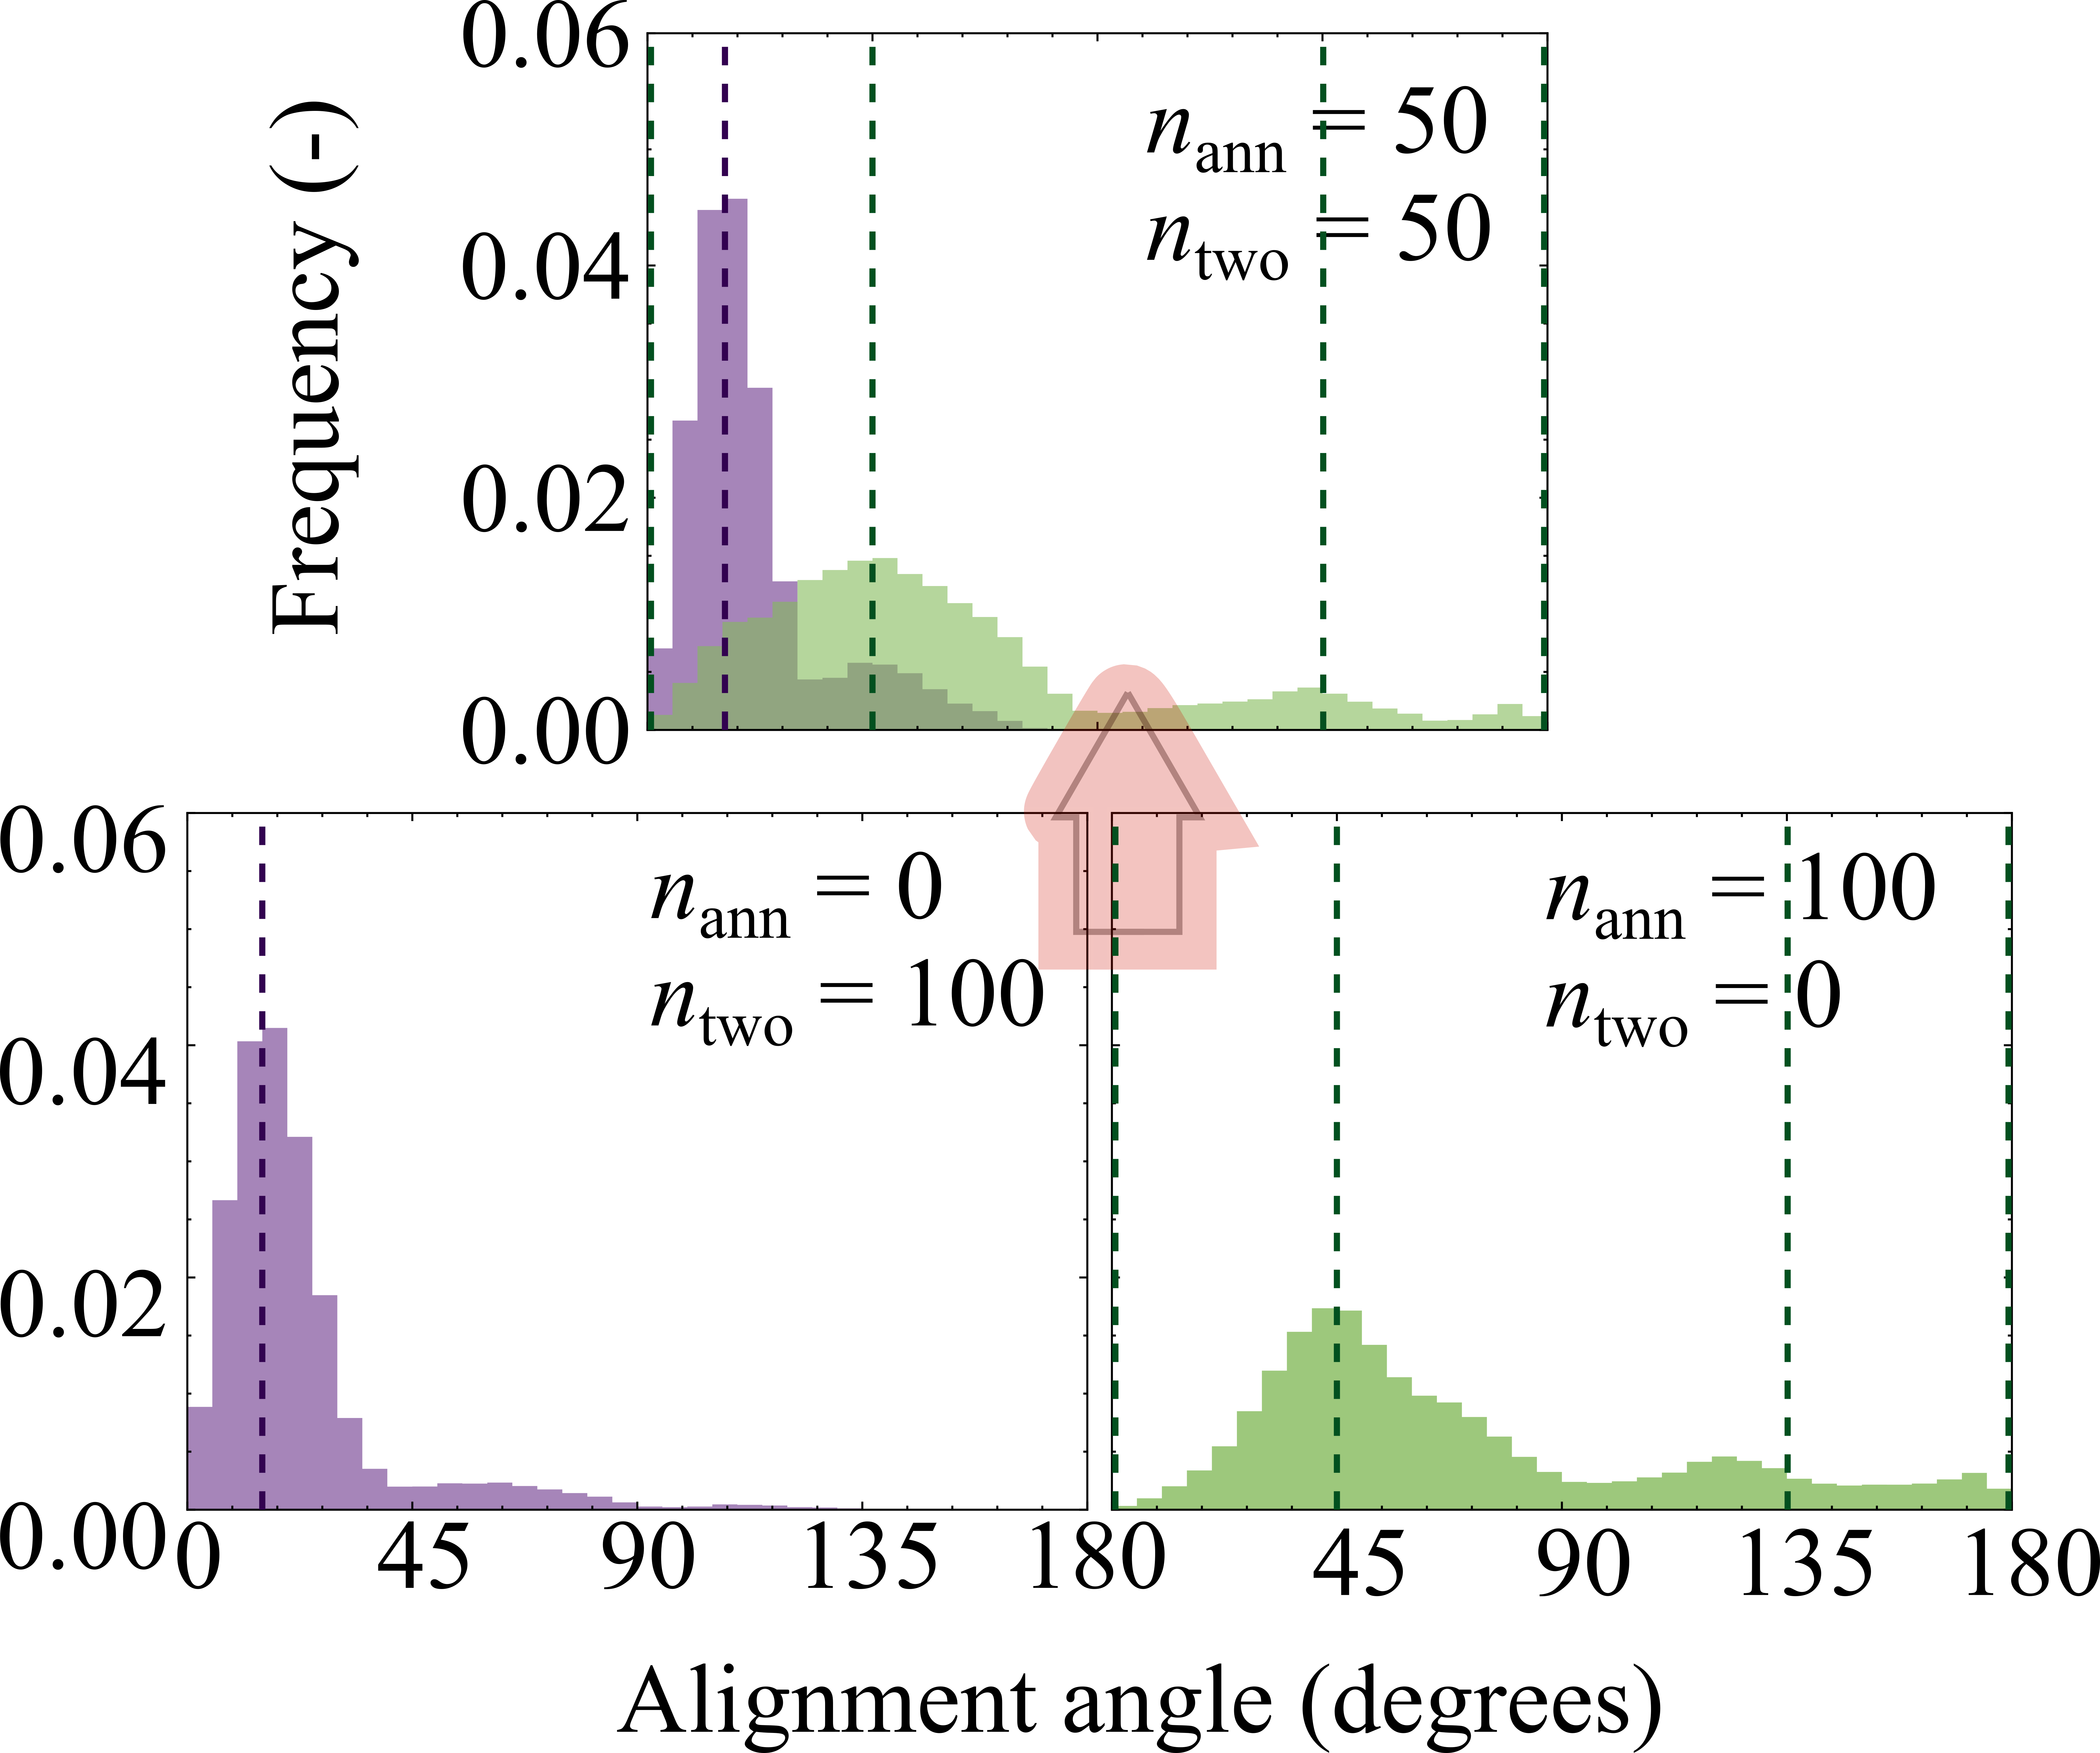
\includegraphics[width=0.5\linewidth]{Figures/alignment_angle_hetero_SI_draft.png}
\caption{Alignment angle distributions for homogeneous and heterogeneous A and B clusters each containing 100 molecules.}
\label{figSI:alignmentangles_100}
\end{figure}
%

% \subsection{Radial distances}
% Table~\ref{tableSI:radialdistances} presents the average equilibrium radial distances for all clusters.  For the homogeneous cases, the two molecule types show similar equilibrium radial distances according to the cluster diameter.  However, in all clusters containing two molecule types the smaller corannulene molecules possess larger radial distances than the larger 2pent15ring molecule.  This is indicative of a core-shell structure in which the larger molecules reside in the cluster core, just as seen in the fPAH clusters \cite{bowal2018partitioning}.
% The addition of the potassium cation(s) also result in significant decreases in the radial distances for both molecule types.
%
% \begin{table}[]
% \centering
% \caption{Equilibrium radial distance, in nm, for all clusters studied}
% \begin{tabular}{lcc}
% \hline
% \multicolumn{1}{l}{\multirow{2}{*}{Cluster}} & \multicolumn{2}{c}{Radial distance} \\ 
% \multicolumn{1}{c}{} & \multicolumn{1}{c}{corannulene} & \multicolumn{1}{c}{2pent15ring} \\ \hline
% ann\_25 & \multicolumn{1}{c}{0.86} & -- \\
% ann\_40 & \multicolumn{1}{c}{1.04} & -- \\
% ann\_50 & \multicolumn{1}{c}{1.11} & -- \\
% ann\_100 & \multicolumn{1}{c}{1.42} & -- \\
% ann\_200 & \multicolumn{1}{c}{1.80} & -- \\ \hline
% two\_25 & \multicolumn{1}{c}{--} & 1.21 \\
% two\_40 & \multicolumn{1}{c}{--} & 1.37 \\
% two\_50 & \multicolumn{1}{c}{--} & 1.40 \\
% two\_100 & \multicolumn{1}{c}{--} & 1.85 \\ \hline
% two\_20\_ann\_20 & \multicolumn{1}{c}{1.28} & 1.14 \\
% two\_50\_ann\_50 & \multicolumn{1}{c}{1.83} & 1.50 \\
% two\_10\_ann\_30 & \multicolumn{1}{c}{1.18} & 0.96 \\
% two\_30\_ann\_10 & \multicolumn{1}{c}{1.50} & 1.25 \\ \hline
% two\_40\_K\_1 & \multicolumn{1}{c}{--} & 1.32 \\
% ann\_40\_K\_1 & \multicolumn{1}{c}{1.02} & -- \\
% ann\_40\_K\_2 & \multicolumn{1}{c}{1.01} & -- \\ \hline
% \end{tabular}
% \label{tableSI:radialdistances}
% \end{table}
%

Figure~\ref{figSI:radialdists_molec} shows the average molecular radial distances for molecule types within clusters. Note that the histograms corresponding to the fPAH clusters [(e) and (f)] are smoothed since these results were taken from an REMD simulation instead of a post-REMD MD simulation at a single temperature.
%
\begin{figure}[!tbh]
\centering
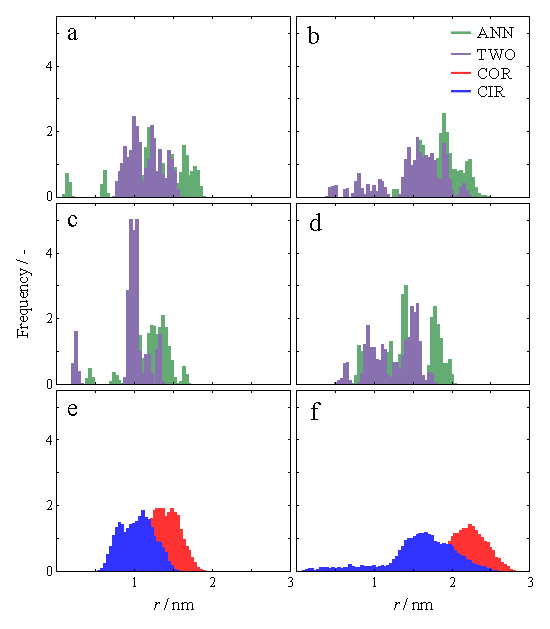
\includegraphics[width=0.5\linewidth]{Figures/molec_histograms.eps}
\caption{Atomic radial distance histograms for (a) two\_20\_ann\_20, (b) two\_50\_ann\_50, (c) two\_10\_ann\_30, (d) two\_30\_ann\_10, and (e) cir\_16\_cor\_16.}
\label{figSI:radialdists_molec}
\end{figure}
%

\newpage